\newif\ifglobal

%%%%%%%%%%%%%%%%%%%%%%%
%%% Compile to view %%%
%%%%%%%%%%%%%%%%%%%%%%%

%%%%%%%%%%%%%%%%%%%%%%%%%%%%%%%%%%%%%%%%%%%%%%%%%%%
%%% Readme:                                     %%%
%%% https://www.overleaf.com/read/bwdjvfjksvjy/ %%%
%%%%%%%%%%%%%%%%%%%%%%%%%%%%%%%%%%%%%%%%%%%%%%%%%%%

% >>> M?: marks a module setting number or important notice

% >>> M4: Set {./relative-path} to external files for this module <<<
\def \modulefiles {./03-ULP}
% To add an external file, use:
% (Replace '---' with actual filename)
% '\input{\modulefiles/tables/---.tex}' for tables
% '\includegraphics{\modulefiles/figures/---}' for figures
% '\subfile{\modulefiles/---}' for register files

% >>> M1: This module is in global project? <<<
% 'YES' - uncomment; 'NO' - comment out
\globaltrue

\ifglobal
    \documentclass[main\_\_EN.tex]{subfiles}

\else
    \documentclass[openany, 10pt]{book}

    % >>> M2: In ./00-shared/preamble-trm-module, also find
    %         settings for visibility of todo notes, watermark <<<
    \usepackage{preamble-trm-module}

    % >>> M3: Temporary labels in English,
    %         you can add your own labels there <<<
    \myexternaldocument{./00-shared/temp-labels-en}

\fi %\ifglobal


\setcounter{secnumdepth}{4}


% Define formatting of parts and chapters in text
\titleformat{\chapter}
  [display]
  {\LARGE\bfseries}
  {\color{AllportsColor}Chapter \thechapter}
  {1em}
  {\color{AllportsColor}}
\titlespacing*{\chapter}{0pt}{0pt}{20pt}

% Define headers
\usepackage{fancyhdr}
\usepackage{lipsum}
\renewcommand{\chaptermark}[1]{\markboth{Chapter\, \thechapter\, \ #1}{}}
\fancypagestyle{plain}{%
  \fancyhead{}%
  %\fancyhead[R]{\Navigation}
  \fancyhead[L]{%
    \nouppercase{%
      \ %
      \normalsize\leftmark
    }%
  }%
}
\pagestyle{plain}


% >>> M5: If this module needs any updates in
% './00-shared/preamble-trm-module.sty'
% (include additional package, etc.), contact your module PM
% or create the file './00-shared/changelog.tex' make the
% necessary updates yourself and document them in this file <<<

% Make text left-aligned and allow latex to break pages naturally, comment out for full justification
\raggedright
\raggedbottom


\begin{document}


% Sets language into which pre-defined bits of text are translated
\selectlanguage{english}

% Do not delete this block
\ifglobal
% Add the following front matter if
% this module is outside of global project
\else
    \InputIfFileExists{readme}{}{}
    \listoftodos
    {\let\clearpage\relax \listofdonetodos}
    \tableofcontents
    %\listoftables
    %\listoffigures
\fi


%%%%%%%%%%%%%%%%%%%%%%%%%
%%% TRM Module Begins %%%
%%%%%%%%%%%%%%%%%%%%%%%%%

\hypertarget{ulp}{}
\chapter{Low-Power CPU}
\label{mod:ulp}

The \chipname{} Low-Power CPU (LP CPU) is a 32-bit processor based upon RISC-V ISA comprising integer (I), multiplication/division (M), atomic (A), and compressed (C) standard extensions. It features ultra-low power consumption and has a 2-stage, in-order, and scalar pipeline. The LP CPU core complex has an interrupt controller (INTC), a debug module (DM), and system bus (SYS BUS) interfaces for memory and peripheral access.

The LP CPU is in sleep mode by default (see Section \ref{sec:sleep}). It can stay powered on when the chip enters Deep-sleep mode (see Chapter \ref{mod:lowpowm} \textit{\nameref{mod:lowpowm}} for details) and can access most peripherals and memories (see Chapter \ref{mod:sysmem} \textit{\nameref{mod:sysmem}} for details). It has two application scenarios:
\begin{itemize}
    \item Power insensitive scenario: When the High-Performance CPU (HP CPU) is active, the LP CPU can assist the HP CPU with some speed- and efficiency-insensitive controls and computations.
    \item Power sensitive scenario: When the HP CPU is in the power-down state to save power, the LP CPU can be woken up to handle some external wake-up events.
\end{itemize}

Figure \ref{figure:ulp-overview} shows the resources accessible to the HP CPU and the LP CPU.

\begin{figure}[!ht ]
    \centering
    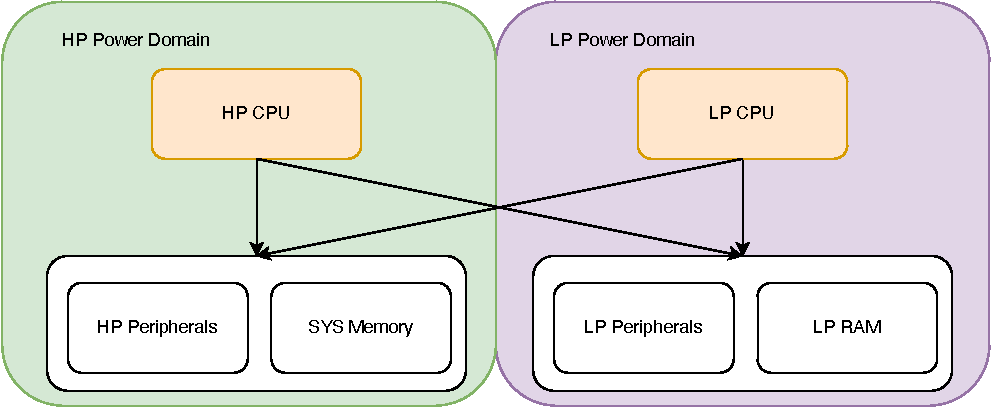
\includegraphics[width=0.7\textwidth]{./03-ULP/figures/03-ULP-lp-core-overview.pdf}
    \caption{LP CPU Overview}
    \label{figure:ulp-overview}
\end{figure}

In the figure above, the HP Power Domain and LP Power Domain can be powered on and off independently. When one domain is powered down, the CPU of the other domain cannot access the resources of that domain. In other words, only when the domain is powered on can its resources be accessed. For more information about power, please refer to the chapter \ref{mod:lowpowm} \textit{\nameref{mod:lowpowm}}.

\section{Features}
\label{sec:ulp-features}

The LP CPU has the following features:

\begin{itemize}
    \item Operating clock frequency up to 20 MHz
    \item One vector interrupt input
    \item Debug module compliant with RISC-V External Debug Support Version 0.13 with external debugger support over an industry-standard JTAG/USB port
    \item Hardware trigger compliant with RISC-V External Debug Support Version 0.13 with up to 2 breakpoints/watchpoints
    \item 32-bit AHB system bus for peripheral and memory access
    \item Core performance metric events
    \item Able to wake up the HP CPU and send an interrupt to it
    \item Access to HP memory and LP memory
    \item Access to the entire peripheral address space

\end{itemize}

\section{Configuration and Status Registers (CSRs)}
\hypertarget{ulp-reg-summ}{}
\subsection{Register Summary}
\label{sec:ulp-reg-summ}


Below is a list of CSRs available to the CPU. Except for the custom performance counter CSRs, all the implemented CSRs follow the standard mapping of bit fields as described in the RISC\-/V Instruction Set Manual, Volume II: Privileged Architecture, Version 1.10. It must be noted that even among the standard CSRs, not all bit fields have been implemented, limited by the subset of features implemented in the CPU. Refer to the next section for a detailed description of the subset of fields implemented under each of these CSRs.

The abbreviations given in Column \textbf{Access} are explained in Section \hyperref[glossary-access-types]{\textit{Access Types for Registers}}.

\subfile{\modulefiles/03-ULP-reg-summ__EN}

Note that if write, set, or clear operation is attempted on any of the read-only (RO) CSRs indicated in the above table, the CPU will generate an illegal instruction exception.

\subsection{Registers}

For how to program reserved fields, please refer to Section \hyperref[programming-reserved-field]{\textit{Programming Reserved Register Field}}.

\subfile{\modulefiles/03-ULP-reg__EN}


\section{Interrupts and Exceptions}

The LP CPU handles interrupts and exceptions according to RISC\-/V Instruction Set Manual, Volume II: Privileged Architecture, Version 1.10. After entering an interrupt/exception handler, the CPU:
\begin{itemize}
    \item Saves the current program counter (PC) value to the \hyperref[regdesc:LPMEPC]{mepc} CSR
    \item Copies the state of \hyperref[fielddesc:LPMSTATUSMIE]{MIE} of \hyperref[regdesc:LPMSTATUS]{mstatus} to \hyperref[fielddesc:LPMSTATUSMPIE]{MPIE} of \hyperref[regdesc:LPMSTATUS]{mstatus}
    \item Saves the current privileged mode to \hyperref[fielddesc:LPMSTATUSMPP]{MPP} of \hyperref[regdesc:LPMSTATUS]{mstatus}
    \item Clears \hyperref[fielddesc:LPMSTATUSMIE]{MIE} of \hyperref[regdesc:LPMSTATUS]{mstatus}
    \item Toggles the privileged mode to machine mode (M mode)
    \item Jumps to the handler address
        \begin{itemize}
            \item For exceptions, the handler address is the base address of the vector table in the \hyperref[regdesc:LPMTVEC]{mtvec} CSR.
            \item For interrupts, the handler address is $mtvec + 4*30$.
        \end{itemize}
    \item After the mret instruction is executed, the core jumps to the PC saved in the \hyperref[regdesc:LPMEPC]{mepc} CSR and restores the value of \hyperref[fielddesc:LPMSTATUSMPIE]{MPIE} of \hyperref[regdesc:LPMSTATUS]{mstatus} to \hyperref[fielddesc:LPMSTATUSMIE]{MIE} of \hyperref[regdesc:LPMSTATUS]{mstatus} and the privileged mode to that configured by \hyperref[fielddesc:LPMSTATUSMPP]{MPP}.
\end{itemize}

When the core starts up, the base address of the vector table is initialized to the boot address 0x50000000. After startup, the base address can be changed by writing to the \hyperref[regdesc:LPMTVEC]{mtvec} CSR. For more information about CSRs, see Section \ref{sec:ulp-reg-summ}.

The core fetches instructions from address 0x50000080 after reset.

\subsection{Interrupts}\label{sec:ulp-intr}

The \chipname{} LP CPU supports only one interrupt entry, to which all interrupt events jump. The LP CPU supports the following peripheral interrupt sources:
\begin{itemize}
    \item \hyperref[mod:lowpowm]{Power Management Unit (PMU)}
    \item \hyperref[mod:lowpowm]{Low-Power Timer (RTC\_TIMER)}
    \item \hyperref[mod:uart]{Low-Power UART (LP\_UART)}
    \item \hyperref[mod:i2c]{Low-Power I2C (LP\_I2C)}
    \item \hyperref[mod:iomuxgpio]{Low-Power IO MUX (LP IO MUX)}
\end{itemize}

For more information on those peripheral interrupts, please refer to the corresponding chapter.

\subsection{Interrupt Handling}

By default, interrupts are disabled globally because the \hyperref[fielddesc:LPMSTATUSMIE]{MIE} bit in \hyperref[regdesc:LPMSTATUS]{mstatus} has a reset value of 0. Software must set this bit to enable global interrupts.

\begin{enumerate}
    \item Enable interrupts
        \begin{itemize}
            \item To enable interrupts globally, set the \hyperref[fielddesc:LPMSTATUSMIE]{MIE} bit of \hyperref[regdesc:LPMSTATUS]{mstatus}.
            \item To enable Interrupt 30, set the 30th bit of \hyperref[regdesc:LPMIE]{mie} CSR.
        \end{itemize}
    \item After interrupts are enabled, the LP CPU can respond to interrupts. It also needs to configure interrupts of the peripherals so that they can send an interrupt signal to the LP CPU.
    \item After the interrupt is triggered, the LP CPU jumps to $mtvec + 4*30$.
    \item After enterring the interrupt handler, users need to read \hyperref[regdesc:LPPERIINTERRUPTSOURCEREG]{LPPERI\_INTERRUPT\_SOURCE\_REG} to get the peripheral that triggered the interrupt and process the interrupt. Note that if the interrupts are triggered by multiple peripherals, the CPU will process them one by one in sequence until none is left. If not all interrupts are processed, the CPU will enter the interrupt handler again.
    \item To clear interrupts, just clear the interrupt signal of the peripheral.
\end{enumerate}

\subsection{Exceptions}

The LP CPU supports the RISC-V standard exceptions and can trigger the following exceptions:

\begin{longtable}[c]{|l|L{8 cm}|}
    \caption{LP CPU Exception Causes}\label{tab:ulp-exc-cause}\\\hline
    \rowcolor{lightgray}
    Exception ID & Description \\\hline
    \endfirsthead
    \hline
    \rowcolor{lightgray}
        Exception ID & Description \\\hline
    \endhead
    \endfoot

    2 & Illegal instructions \\\hline
    3 & Breakpoints (EBREAK) \\\hline
    6 & Misaligned atomic instructions \\\hline

\end{longtable}


\section{Debugging}

This section describes how to debug and test the LP CPU. Debug support is provided through standard JTAG pins and complies with RISC-V External Debug Support Version 0.13.

For \chipname{} system debugging overview, please refer to Chapter \ref{mod:riscvcpu} \textit{\nameref{mod:riscvcpu}} > Figure \ref{fig:riscvcpu-dbg-sys-overview}.

The user interacts with the Debug Host (e.g., laptop), which is running a debugger (e.g., gdb). The debugger communicates with a Debug Translator (e.g., OpenOCD, which may include a hardware driver) to communicate with Debug Transport Hardware (e.g., ESP-Prog adapter). The Debug Transport Hardware connects the Debug Host to the CPU's Debug Transport Module (DTM) through a standard JTAG interface. The DTM provides access to the debug module (DM) using the Debug Module Interface (DMI).

\chipname{} features two DTMs interconnected in a daisy-chain configuration. Specifically, TAP0 connects to the HP CPU, and TAP1 is dedicated to the LP CPU.

The HP DM can debug the HP CPU and the LP DM the LP CPU.


The LP CPU implements four registers for core debugging: \hyperref[regdesc:LPDCSR]{dcsr}, \hyperref[regdesc:LPDPC]{dpc}, \hyperref[regdesc:LPDSCRATCH0]{dscratch0}, and \hyperref[regdesc:LPDSCRATCH1]{dscratch1}. All of those registers can only be accessed from debug mode. If software attempts to access them when the LP CPU is not in debug mode, an illegal instruction exception will be triggered.

\subsection{Features}
The Low-Power CPU has the following debugging features:
\begin{itemize}
    \item {Provides necessary information about the implementation to the debugger.}
    \item {Allows the CPU core to be halted and resumed.}
    \item {CPU core registers (including CSRs) can be read/written by the debugger.}
    \item {CPU core can be reset through the debugger.}
    \item {CPU can be halted on software breakpoint (planted breakpoint instruction).}
    \item {Hardware single-stepping.}
    \item {Two hardware triggers (which can be used as breakpoints/watchpoints). See Section \ref{sec:ulp-trigger} for details.}
\end{itemize}

\subsection{Functional Description}
The debugging mechanism adheres to the specification RISC-V External Debug Support Version 0.13. For a detailed description of the debugging features, refer to the specification.

According to the specification, a hart can be in the following states: nonexistent, unavail, running, and halted. By default, the LP CPU is in the unavail state. To connect the LP CPU for debugging, users need to clear the state by configuring the \hyperref[regdesc:LPPERICPUREG]{LPPERI\_CPU\_REG} register.

\subsection{Register Summary}

The following table lists the debug CSRs supported for the LP CPU.

The abbreviations given in Column \textbf{Access} are explained in Section \hyperref[glossary-access-types]{\textit{Access Types for Registers}}.

\subfile{\modulefiles/03-ULP-DBG-reg-summ__EN}

All debug module registers are implemented in accordance with the specification RISC-V External Debug Support Version 0.13. For more information, refer to the specification.

\subsection{Registers}
%%%%%%%%%
The following is a detailed description of the debug CSR supported by the LP CPU.

For how to program reserved fields, please refer to Section \hyperref[programming-reserved-field]{\textit{Programming Reserved Register Field}}.

\subfile{\modulefiles/03-ULP-DBG-reg__EN}


\section{Hardware Trigger}\label{sec:ulp-trigger}

\subsection{Features}
Hardware Trigger module provides breakpoint and watchpoint capability for debugging. It has the following features:

\begin{itemize}
    \item Two independent trigger units
    \item Configurable unit to match the address of the program counter
    \item Able to halt execution and transfer control to the debugger

\end{itemize}

\subsection{Functional Description}
\label{sec:ulp-hwt-func-descr}

The hardware trigger module provides three CSRs. See Section \ref{sec:ulp-hwt-reg-summ} for details. Among these, \hyperref[regdesc:LPTDATA1]{tdata1} and \hyperref[regdesc:LPTDATA2]{tdata2} are abstract CSRs, which means they are shadow registers for accessing internal registers in the trigger units, one at a time.

To select a specific trigger unit, the corresponding number (0-1) needs to be written to the \hyperref[regdesc:LPTSELECT]{tselect} CSR. When a valid value is written, the abstract CSRs, \hyperref[regdesc:LPTDATA1]{tdata1} and \hyperref[regdesc:LPTDATA2]{tdata2}, automatically match the internal registers of the trigger unit. Each trigger unit has two internal registers, namely \hyperref[regdesc:LPMCONTROL]{mcontrol} and \hyperref[regdesc:LPMADDRESS]{maddress}, which are mapped to \hyperref[regdesc:LPTDATA1]{tdata1} and \hyperref[regdesc:LPTDATA2]{tdata2}, respectively.

Writing a value more than 1 to \hyperref[regdesc:LPTSELECT]{tselect} will set \hyperref[regdesc:LPTSELECT]{tselect} to 1.

Since software or debugger may need to know the type of the selected trigger to correctly interpret \hyperref[regdesc:LPTDATA1]{tdata1} and \hyperref[regdesc:LPTDATA2]{tdata2}, the 4-bit field (31-28) of \hyperref[regdesc:LPTDATA1]{tdata1} encodes the type of the selected trigger. This type field is read-only and always provides a value of 0x2 for every trigger, which stands for support for address and data matching. Hence, it is inferred that \hyperref[regdesc:LPTDATA1]{tdata1} and \hyperref[regdesc:LPTDATA2]{tdata2} are to be interpreted as fields of \hyperref[regdesc:LPMCONTROL]{mcontrol} and \hyperref[regdesc:LPMADDRESS]{maddress}, respectively. The specification RISC-V External Debug Support Version 0.13 provides information on other possible values, but the trigger module only supports the 0x2 type.

Once a trigger unit has been chosen by writing its index to \hyperref[regdesc:LPTSELECT]{tselect}, it will become possible to configure it by setting the appropriate bits in \hyperref[regdesc:LPMCONTROL]{mcontrol} CSR (\hyperref[regdesc:LPTDATA1]{tdata1}) and writing the target address to \hyperref[regdesc:LPMADDRESS]{maddress} CSR (\hyperref[regdesc:LPTDATA2]{tdata2}).


\subsection{Trigger Execution Flow}
\label{sec:ulp-hwt-suggest-op}

When a hart is halted and enters debug mode due to the firing of a trigger (\hyperref[fielddesc:LPMCONTROLACTION]{action} = 1):
\begin{itemize}
    \item \hyperref[regdesc:LPDPC]{dpc} is set to the current PC in the decoding phase
    \item The cause field in \hyperref[regdesc:LPDCSR]{dcsr} is set to 2, which means halt due to trigger
\end{itemize}


\subsection{Register Summary}
\label{sec:ulp-hwt-reg-summ}

Below is a list of Trigger Module CSRs supported by the CPU. These are only accessible from machine mode.

The abbreviations given in Column \textbf{Access} are explained in Section \hyperref[glossary-access-types]{\textit{Access Types for Registers}}.

\subfile{\modulefiles/03-ULP-Trigger-reg-summ__EN}

\subsection{Registers}
\label{sec:ulp-hwt-reg}

For how to program reserved fields, please refer to Section \hyperref[programming-reserved-field]{\textit{Programming Reserved Register Field}}.

\subfile{\modulefiles/03-ULP-Trigger-reg__EN}


\section{Performance Counter}

The LP CPU implements a clock cycle counter \hyperref[regdesc:LPMCYCLE]{mcycle(h)}, an instruction counter \hyperref[regdesc:LPMINSTRET]{minstret(h)}, and 10 event counters \hyperref[regdesc:LPMHPMCOUNTER]{mhpmcounter\regindex{n}(\regindex{n}:3-12)}. The clock cycle counter and instruction counter are always available and each is 64-bit wide. Other performance counters are 40-bit wide each.

By default, all counters are enabled after reset. A counter can be enabled or disabled individually via the corresponding bit in the \hyperref[regdesc:LPMCOUNTINHIBIT]{mcountinhibit} CSR.

As shown in Table \ref{tab:ulp-pccr}, each counter is dedicated to counting a particular event.

\begin{longtable}[c]{|l|l|}
    \caption{Performance Counter}\label{tab:ulp-pccr}\\\hline
    \rowcolor{lightgray}
    Counter & Counted Event \\\hline
    \endfirsthead
    \hline
    \rowcolor{lightgray}
    Counter & Counted Event \\\hline
    \endhead
    \endfoot

    mcycle & Clock cycles \\\hline
    minstret & The number of instructions \\\hline
    mhpmcounter3 & Wait cycles for memory access \\\hline
    mhpmcounter4 & Wait cycles for fetching instructions \\\hline
    mhpmcounter5 & The number of memory read operations. An unaligned read is counted as two.  \\\hline

    mhpmcounter6 & The number of memory write operations. An unaligned write is counted as two. \\\hline
    mhpmcounter7 & The number of unconditional jump instructions (jal, jr, jalr) \\\hline
    mhpmcounter8 & The number of branch instructions \\\hline
    mhpmcounter9 &  The number of taken branch instructions \\\hline
    mhpmcounter10 & The number of compressed instructions \\\hline
    mhpmcounter11 & Wait cycles for multiplication instructions \\\hline
    mhpmcounter12 & Wait cycles for division instructions \\\hline

\end{longtable}

\section{System Access}


\subsection{Memory Access}

The \chipname{} LP CPU can access LP SRAM and HP SRAM. For more information, please refer to Section \ref{mod:sysmem} \textit{\nameref{mod:sysmem}}.
\begin{itemize}
    \item LP SRAM: 16 KB starting from 0x5000\_0000 to 0x5000\_3FFF, where you can fetch instructions, read data, write data, etc.
    \item HP SRAM: 384 KB starting from 0x4080\_0000 to 0x4085\_FFFF, where you can fetch instructions, read data, write data, etc.
\end{itemize}

\begin{tiplisting}
The LP CPU has a high latency to access the HP SRAM, but can access the LP SRAM with no latency.
\end{tiplisting}

The LP CPU supports the atomic instruction set. Both the LP CPU and the HP CPU can access memory through atomic instructions, thus achieving atomicity of memory access. For details on the atomic instruction set, please refer to RISC-V Instruction Set Manual Volume I: Unprivileged ISA, Version 2.2.

Note that only HP SRAM supports atomic access from HP CPU and LP CPU.

\subsection{Peripheral Access}

Table \ref{tab:sysmem-base-address} in Chapter \ref{mod:sysmem} \textit{\nameref{mod:sysmem}} lists the peripherals accessible by the LP CPU and their base addresses.

\section{Event Task Matrix Feature}
\label{sec:etm-func}

The LP CPU on \chipname{} supports the Event Task Matrix (ETM) function, which allows LP CPU's ETM tasks to be triggered by any peripherals' ETM events, or LP CPU's ETM events to trigger any peripherals' ETM tasks. This section introduces the ETM tasks and events related to the LP CPU. For more information, please refer to Chapter \ref{mod:evntaskmatrix} \nameref{mod:evntaskmatrix}.

LP CPU can receive the following ETM task:

\begin{itemize}
    \item ULP\_TASK\_WAKEUP\_CPU: Wakes up the LP CPU.
\end{itemize}

LP CPU can generate the following ETM events:

\begin{itemize}
    \item ULP\_EVT\_ERR\_INTR: Indicates that an LP CPU exception occurs.
    \item ULP\_EVT\_START\_INTR: Indicates that the LP CPU clock is turned on.
\end{itemize}


\section{Sleep and Wake-Up Process}\label{sec:sleep}
\subsection{Features}
\begin{itemize}
    \item Able to sleep, wake up, and operate independently in the low-power system when the HP CPU is working or sleeping
    \item Able to actively configure registers to enter the sleep status based on software operating status
    \item Wake-up events:
    \begin{itemize}
        \item The HP CPU setting the register \hyperref[fielddesc:PMUHPTRIGGERLP]{PMU\_HP\_TRIGGER\_LP}
        \item The interrupt state of the LP IO
        \item ETM events
        \item The RTC timer timeout
        \item The LP UART receiving a certain number of RX pulses when \hyperref[fielddesc:LPPERILPUARTWAKEUPEN]{LPPERI\_LP\_UART\_WAKEUP\_EN} is enabled
   \end{itemize}
\end{itemize}

\subsection{Process}
The LP CPU is in sleep by default and its wake-up module follows the process below to wake it up for work and make it sleep.

To configure wake-up sources, please refer to Table \ref{tab:ulp-wake-sources}.

\begin{figure}[!ht ]
    \centering
    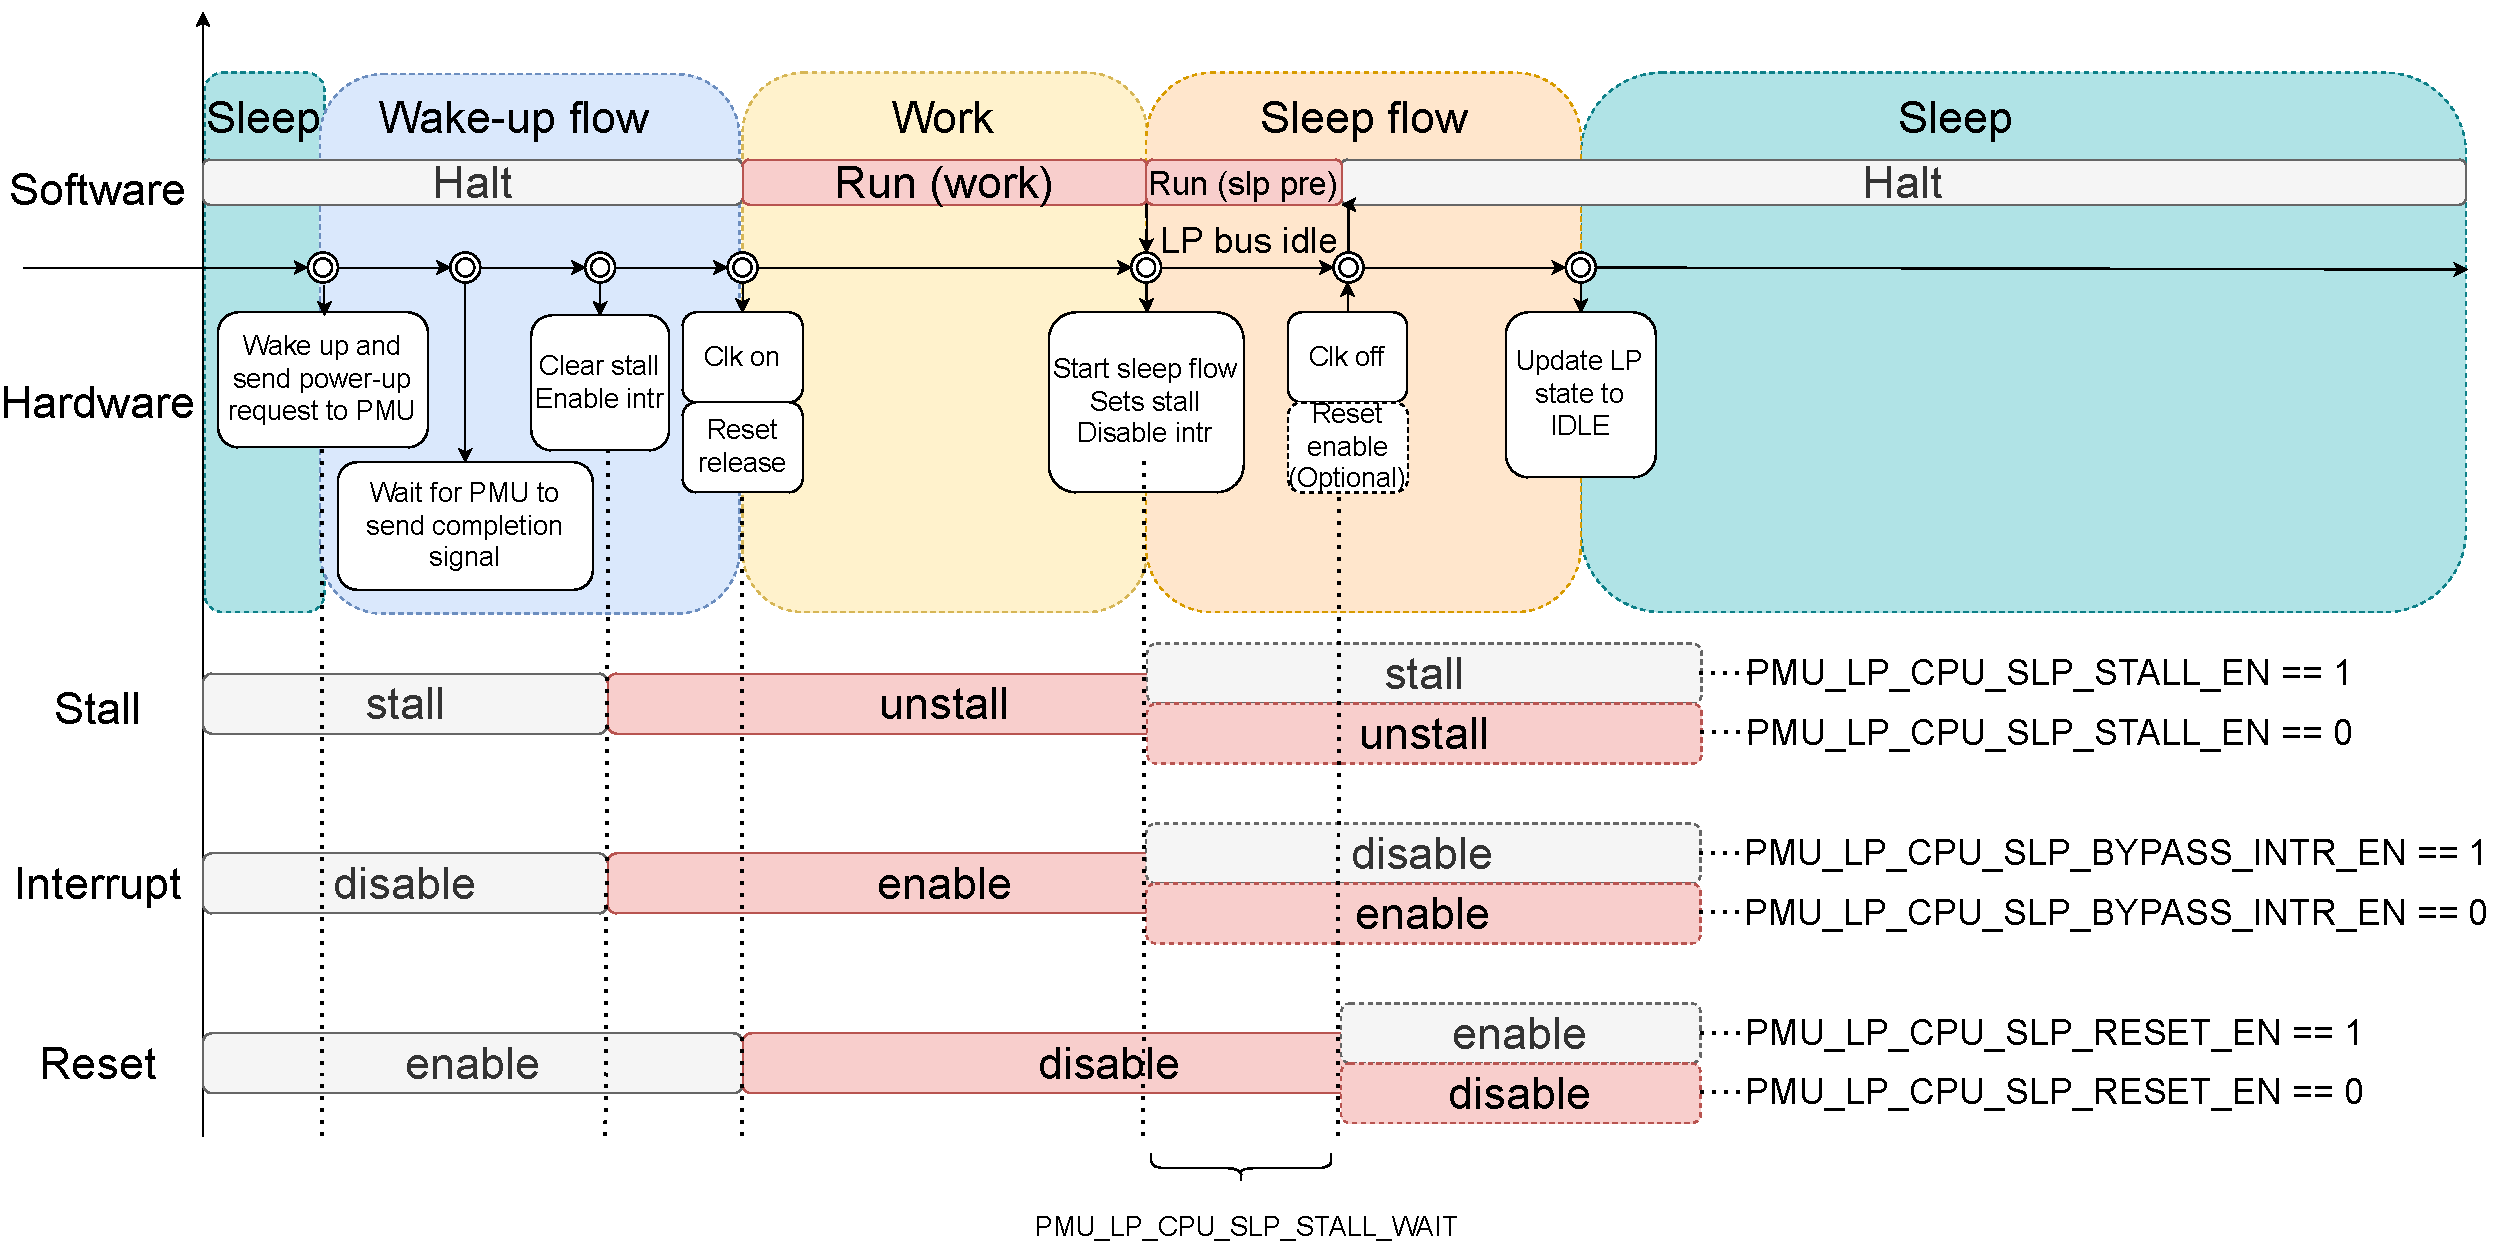
\includegraphics[width=1.0\textwidth]{./03-ULP/figures/03-ULP-lp-core-sleep-wake-flow.pdf}
    \caption{Wake-Up and Sleep Flow of LP CPU}
    \label{figure:ulp-overvew}
\end{figure}

The first startup of the LP CPU after power-up depends on the wake-up enable and wake-up source configuration by the HP CPU.

\begin{itemize}
    \item Initialization of the LP CPU
         \begin{itemize}
         \item Initialize the LP memory.
         \item Start the LP CPU. Since the startup of the LP CPU depends on the wake-up process, it is recommended to use the \hyperref[fielddesc:PMUHPTRIGGERLP]{PMU\_HP\_TRIGGER\_LP} register to start the initialization of the LP CPU in the following way:
             \begin{itemize}
             \item Set \hyperref[fielddesc:PMULPCPUWAKEUPEN]{PMU\_LP\_CPU\_WAKEUP\_EN} to 0x1
             \item Set \hyperref[fielddesc:PMUHPTRIGGERLP]{PMU\_HP\_TRIGGER\_LP} to 0x1
             \item The LP CPU will go through the wake-up process to start running
             \end{itemize}
         \end{itemize}
    \item Wake-up process:
    \begin{itemize}
     \item The wake-up module receives a wake-up signal and sends a power-up request to the PMU.
     \item If the current power consumption state (clock, power supply, etc.) meets the requirements of the LP CPU, the PMU will immediately reply with the completion signal. Otherwise, it will adjust the power consumption state before replying with the completion signal.
     \item The wake-up module disables the STALL state of the LP CPU and enables interrupt receiving.
     \item The wake-up module starts the clock, releases reset (ignore this step if reset is not enabled for sleep), and starts working.
   \end{itemize}

    \item Sleep process:
    \begin{itemize}
    \item The LP CPU configures the register \hyperref[fielddesc:PMULPCPUSLEEPREQ]{PMU\_LP\_CPU\_SLEEP\_REQ} to enable the wake-up module to start the sleep process.
    \item If \hyperref[fielddesc:PMULPCPUSLPSTALLEN]{PMU\_LP\_CPU\_SLP\_STALL\_EN} is 1, the wake-up module enables the STALL state of the LP CPU. If it is 0, the module does not enable that state.
    \item The wake-up module waits for \hyperref[fielddesc:PMULPCPUSLPSTALLWAIT]{PMU\_LP\_CPU\_SLP\_STALL\_WAIT} LP CPU clock cycles, and then turns off the LP CPU clock. If \hyperref[fielddesc:PMULPCPUSLPRESETEN]{PMU\_LP\_CPU\_SLP\_RESET\_EN} is 1, the module enables reset of the LP CPU.
   \end{itemize}
   \end{itemize}



\subsection{Wake-Up Sources}

    \begin{table}[H]
    \centering
    \caption{Wake Sources}
    \label{tab:ulp-wake-sources}
    \begin{threeparttable}
    \begin{tabular}{| l | l | m{7cm}|}
    \hline
    \rowcolor{lightgray}
    Register Value \tnote{1} & Wake-Up Source & Description  \\\hline

    0x1 & Register \hyperref[fielddesc:PMUHPTRIGGERLP]{PMU\_HP\_TRIGGER\_LP} & The HP CPU sets the register \hyperref[fielddesc:PMUHPTRIGGERLP]{PMU\_HP\_TRIGGER\_LP} to wake up the LP CPU, and sets \hyperref[fielddesc:PMUHPSWTRIGGERINTCLR]{PMU\_HP\_SW\_TRIGGER\_INT\_CLR} to clear this wake-up source.\\\hline
    0x2 & LP UART & The LP UART receives a certain number of RX pulses. \hyperref[fielddesc:LPPERILPUARTWAKEUPEN]{LPPERI\_LP\_UART\_WAKEUP\_EN} needs to be enabled. For more information, please refer to Chapter \ref{mod:uart} \textit{\nameref{mod:uart}}. \\\hline
    0x4 & LP IO & This wake-up source uses the LP IO interrupt status register signal. For more information, please refer to Chapter \ref{mod:iomuxgpio} \textit{\nameref{mod:iomuxgpio}}. \\\hline
    0x8 & ETM & Wake-up sources received from ETM can wake up the LP CPU. For more information, please refer to Chapter \ref{mod:evntaskmatrix} \textit{\nameref{mod:evntaskmatrix}}. \\\hline
    0x10 & RTC timer & RTC timer target 1 timeout interrupt control. For more information, please refer to Chapter \ref{mod:lowpowm} \textit{\nameref{mod:lowpowm}}. \\\hline
\end{tabular}
    \begin{tablenotes}
        \item[1] Value of the \hyperref[fielddesc:PMULPCPUWAKEUPEN]{PMU\_LP\_CPU\_WAKEUP\_EN} register
    \end{tablenotes}
    \end{threeparttable}
\end{table}


\section{Register Summary}
\label{sec:ulp-lpperi-reg-summ}
The addresses in this section are relative to Low-Power Peripheral base address provided in Table \ref{tab:sysmem-base-address} in Chapter \ref{mod:sysmem} \textit{\nameref{mod:sysmem}}.

The abbreviations given in Column \textbf{Access} are explained in Section \hyperref[glossary-access-types]{\textit{Access Types for Registers}}.

\subfile{\modulefiles/03-ULP-LPPERI-reg-summ__EN}

%%%%%%%%%%%%%%%%%
%%% Registers %%%
%%%%%%%%%%%%%%%%%

\section{Registers}

For how to program reserved fields, please refer to Section \hyperref[programming-reserved-field]{\textit{Programming Reserved Register Field}}.

The addresses in this section are relative to Low-Power Peripheral base address provided in Table \ref{tab:sysmem-base-address} in Chapter \ref{mod:sysmem} \textit{\nameref{mod:sysmem}}.


\subfile{\modulefiles/03-ULP-LPPERI-reg__EN}

\end{document}
